\documentclass{beamer}
\usetheme{Madrid}
\usecolortheme{beaver}
\title{Mass \& Balance}
\subtitle{Lesson 1}
\author{Alberto Botto Poala}
\institute{AeC Biella}
\date{\today}

\begin{document}

\begin{frame}
\titlepage
\end{frame} 

\begin{frame}
\frametitle{Table of Contents}
\tableofcontents
\end{frame} 

\section{Massa vs Forza Peso}
\begin{frame}
\frametitle{Title}
\textbf{massa}:è una grandezza fisica propria dei corpi materiali che ne determina il comportamento dinamico quando sono soggetti all'influenza di forze esterne.
\begin{figure}
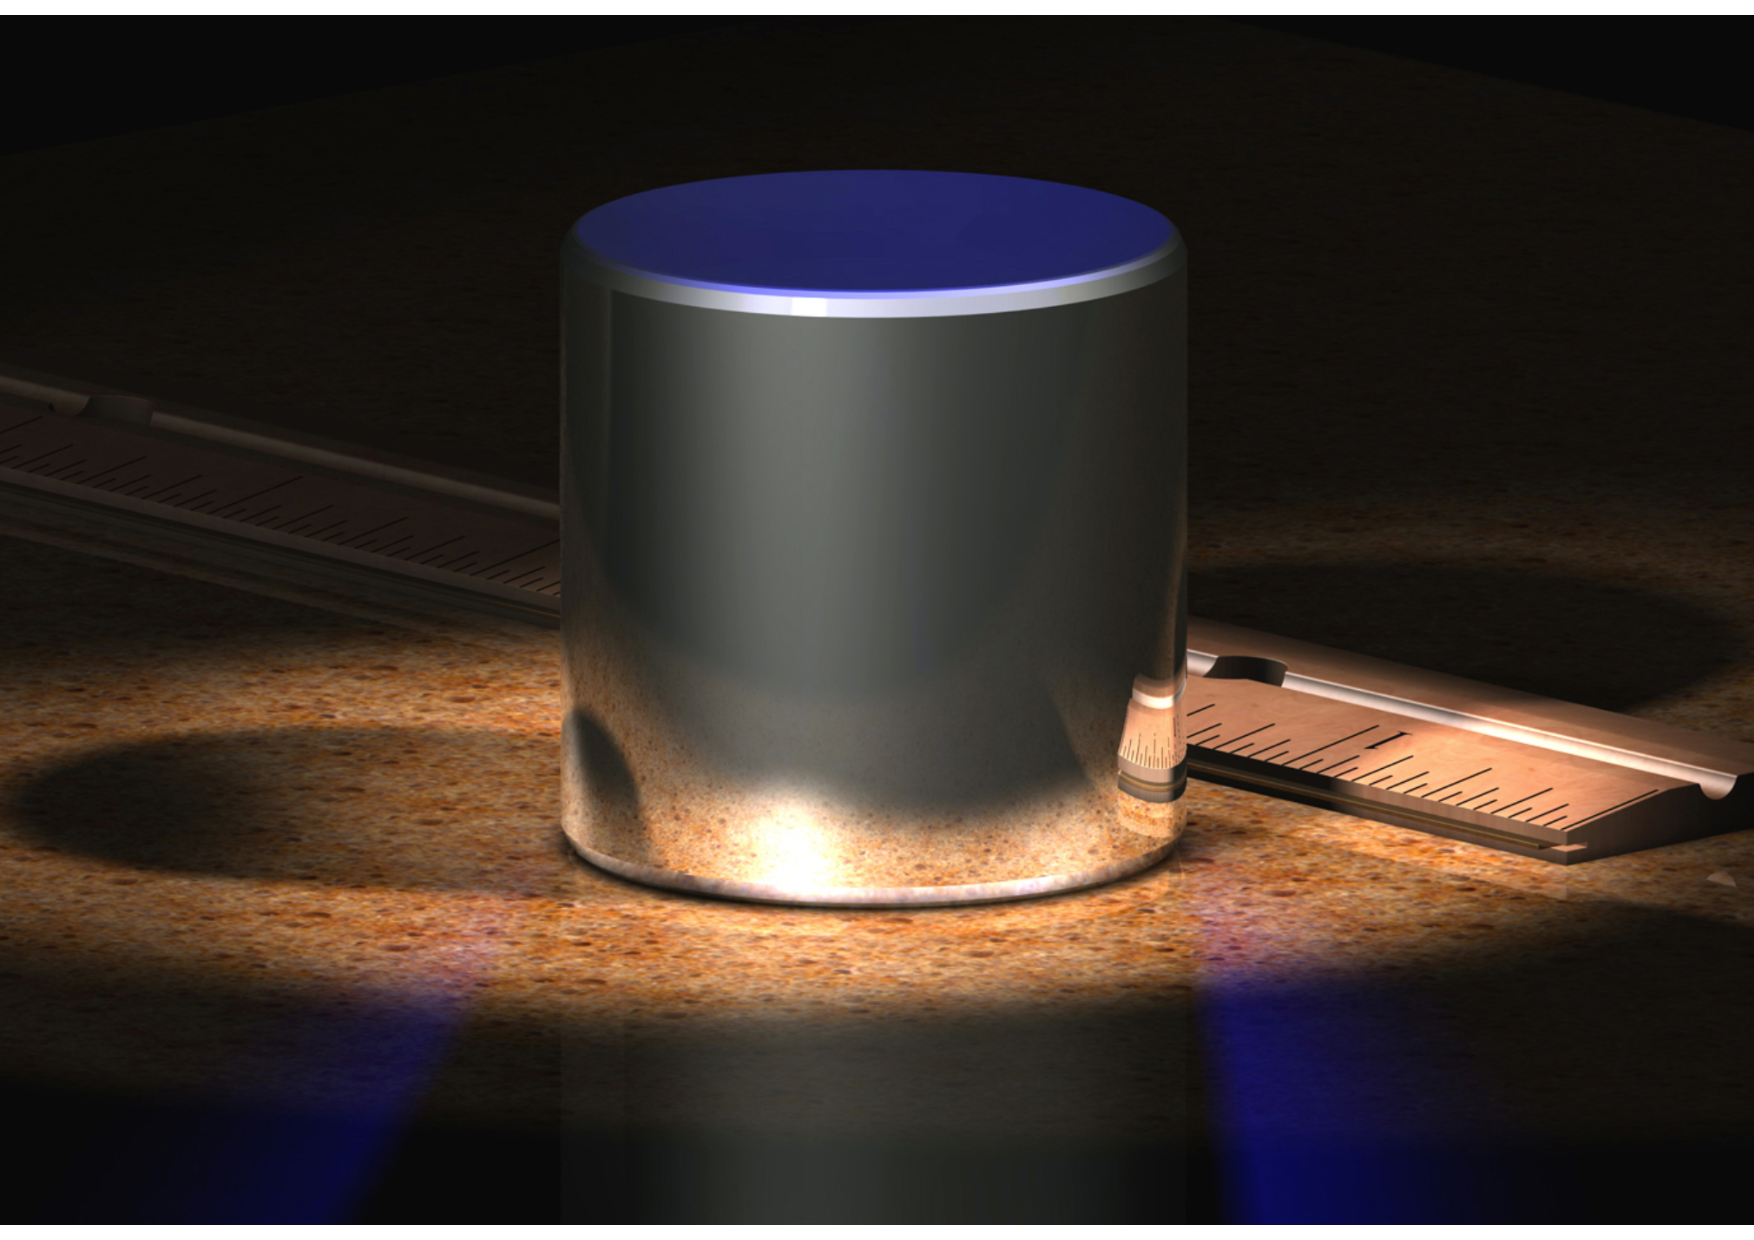
\includegraphics[scale=0.1]{./images/1kg.pdf}
\end{figure}
\end{frame}

\section{Massa vs Momento d'Inerzia}
\end{document}
